% When the state of the system is finished with its reaching phase, the system enters the sliding phase. The sliding phase
% are reached when the systems slides along the manifold heading towards the equilibrium point in origin. One way to do
% this is with a control law as:
% \begin{equation}
%   u = -\beta \left( \vect{x} \right)\up{sign}(s)
% \end{equation}
% Where:
% \begin{alignat}{5}
%        & \beta (\vect{x}) & \hspace{1cm} & \quad\text{is a control gain function} \hspace{1cm} &  & \nonumber \\ 
%        & s                & \hspace{1cm} & \quad\text{is the manifold} \hspace{1cm}            &  & \nonumber
% \end{alignat}
% And:
% \begin{equation}
%   \up{sign}(s) =
%   \begin{cases}
%     -1 & \quad s < 0 \\
%      0 & \quad s = 0 \\
%      1 & \quad s > 0
%   \end{cases}
% \nonumber
% \end{equation}
% \begin{figure}[H]
%   \centering
%   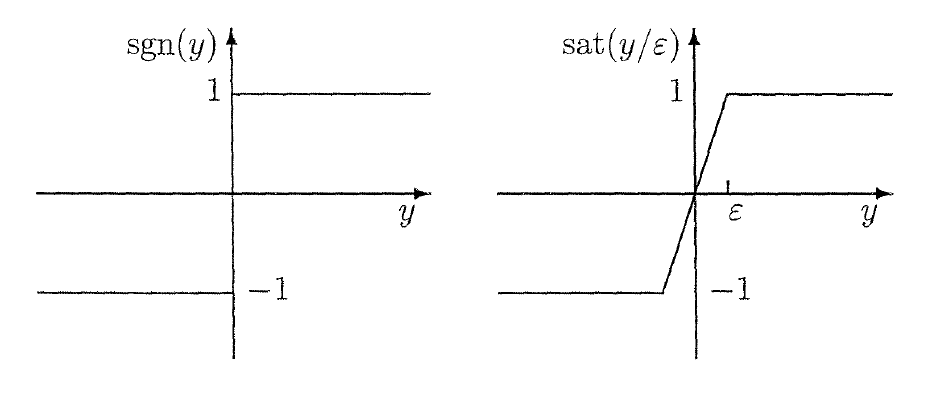
\includegraphics[width=0.6\textwidth]{saturation}
%   \caption{Signum function (left) and the saturation function (right).}
%   \label{fig:sign_sat}
% \end{figure}
In the ideal case the sliding mode control should begin sliding along the sliding surface when reached. In reality, the trajectories will overshoot the sliding surface because of delays in the switching term in the control equation \ref{eq:control_ideal}. This overshoot will result in a ``zig-zag'' motion (oscillations) along the sliding surface because of the rapid sign change in the control. This Chattering downgrades the performance of the control and might even attenuate unmodelled high-frequency dynamics.

In order to reduce chattering and account for imprecision in the system model and disturbances we must insure that the inequality in equation \ref{eq:lyap_dot} still hold with perturbations. We take the control to consist of two parts, a continuous and a switching part where we denote $\hat{h}(x)$ and $\hat{g}(x)$ as the nominal model and $h(x)$ and $g(x)$ as the uncertain model.
\begin{equation}
        u = - \frac{[a_1 x_2 + \hat{h}(x)]}{\hat{g}(x)} + v
\end{equation}
Then the derivative of the sliding surface becomes:
\begin{equation}
        \dot{s} = a_1\left(1 - \frac{c}{\hat{c}}\right) x_2 + \left(\frac{c}{\hat{c}} - 1\right)\hat{a} \sin (\bar{x}_1 - \delta_1) + \left(\frac{c}{\hat{c}}\hat{b} - b\right) x_2 + cv + \xi(t) \doteq \delta(t) + cv
\end{equation}
By taking $V = (1/2) s^2$ we check for the inequality $\dot{V} \leq 0$ is satisfied:
\begin{equation}
        \dot{V} = s\dot{s} = s\delta(x) + scv \leq \vert s \vert \delta(x) + \vert s \vert c v \leq 0
\end{equation}
from this inequality it can be seen that the switching term $v$ should be equal to
\begin{equation}
        v = -\beta(x)\up{sgn(s)}
\end{equation}
where $\beta(x) \geq \varrho(x) + \beta_0$ and $\varrho(x)$ is then the upper bound on the perturbation which satisfies the inequality
% This strategy can, however, give rise to a fair amount of chattering in the system. To alleviate this we define a
% constant, $\epsilon$. The constant $\epsilon$ is used to define a region close to the sliding surface where, when
% within, the sgn$()$ function is replaced with an approximation of a discontinous function - a saturation function.
% We can divide the control into a continuous and a switching part
\begin{equation}
        \left \vert \frac{\delta(t)}{c} \right\vert \leq \varrho(x)
\end{equation}
For the system $\varrho(x)$ is calculated to be
\begin{equation}
        \begin{split}
                \left \vert \frac{\delta(t)}{c} \right\vert &= \left \vert \frac{\hat{a}(\hat{c}-c)}{c\hat{c}} \right \vert \vert \sin (\bar{x}_1 - \delta_1) \vert + \left \vert \frac{a_1 - b}{c} + \frac{\hat{b} - a_1}{\hat{c}} \right \vert \vert x_2 \vert + \left\vert \frac{\xi(t)}{c}\right\vert \\
                &\leq 1576 \vert \bar{x}_1-\delta_1 \vert + 615.2\vert x_2 \vert + 421.38  \leq \varrho(x)
        \end{split}
\end{equation}
In order to reduce the chattering further we replace the sign function in the control with a saturation function. The saturation function is an approximation of a discontinuous function which in the boundary $\vert s \vert \leq \epsilon$ function as a gain and the control becomes
\begin{equation}
  u = -\beta\left( x \right) \up{sat}\left( \frac{s}{\epsilon} \right)
\end{equation}
Where:
\begin{equation}
  \up{sat}\left( \frac{s}{\epsilon} \right) =
  \begin{cases}
    \frac{s}{\epsilon} &\quad \text{if $\vert\frac{s}{\epsilon}\vert$ $\leq$ 1} \\[2mm]
    \up{sgn}\left( \frac{s}{\epsilon} \right) &\quad \text{if $\vert \frac{s}{\epsilon}\vert$ $>$ 1}
  \end{cases}
\end{equation}
The control is then given as
\begin{equation}
        u = -\beta(x)\up{sat}\left(\frac{s}{\epsilon}\right) =  -\left[ 1576 \vert \bar{x}_1-\delta_1 \vert + 615.2\vert x_2 \vert + 422 \right]\up{sat}\left(\frac{s}{\epsilon}\right)
\end{equation}
% where
% \begin{equation}
%         \beta(x) \geq \varrho(x) + \beta_0
% \end{equation}